\setlength{\parskip}{1pt} %% ESPAÇO DEPOIS DE 6pt
\pagenumbering{arabic}  %% PAGINAÇÃO INICIA AQUI
\setcounter{page}{16} % Reiniciar contagem de página para 1
%\pagestyle{plain} % Restaurar numeração de página com estilo "plain"
\clearpage
\pagestyle{fancy}



\section{Introdu{\c c}{\~a}o} \label{sec:int}

%\subsection{Contextualiza\c c\~ao} \label{subsec:contexto}

O acesso à água potável é vital para a saúde e bem-estar das pessoas, sendo um requisito fundamental para a sobrevivência e o desenvolvimento humano. A água potável é essencial para a higiene pessoal, a preparação de alimentos e a prevenção de doenças transmitidas pela água. Além disso, é um componente crucial para o funcionamento adequado de sistemas de saneamento básico. O acesso a água limpa não apenas reduz significativamente a incidência de doenças, mas também promove o crescimento econômico, a educação e a igualdade. Garantir o acesso universal à água potável não apenas salva vidas, mas também contribui para a construção de comunidades saudáveis e sustentáveis em todo o mundo. Os recursos d'água potável estão tornando-se mais escassos em algumas comunidades, em parte devido à crescente procura d'água potável em regiões urbanas, à pobreza de técnicas de gestão d'águas residuais e as secas ou enchentes induzidas pelo clima
\cite{10.2166/wp.2022.071}.

Dada a crescente escassez d'água os órgãos que gerenciam tais recursos recomendam a implementação de novas iniciativas para expandir seus portfólios locais e regionais d'água, incluindo a reutilização d'águas residuais tratadas para fins potáveis para evitar a escassez d'água, questões que poderão piorar drasticamente nas próximas décadas \cite{BARNES2023139587}. A reutilização d'águas residuais tratadas (RART) para fins potáveis ajuda a aliviar o uso das águas superficiais e subterrâneas locais que estão relacionadas com preocupações de escassez. Ao reutilizar águas residuais, as comunidades tornam-se menos dependem dos recursos hídricos disponíveis localmente e operam de forma mais local, girando a economia circular da água centrada \cite{TSATSOU2023136325}. Algumas cidades conseguiram implementar este sistema RART para aumentar o abastecimento local d'água potável, porém no Brasil ainda não temos isto de forma efetiva, então uma possibilidade é fazer previsão da demanda de tal forma que o abastecimento para a população não seja descontinuado. 

O presente estudo envolve dados de abastecimento d'água da cidade de Curitiba no Bairro Alto entre os anos de $2018$ e $2020$. No entanto, vale destacar, que durante o ano de $2022$, os habitantes de Curitiba enfrentaram escassez d'água, sendo necessário implementar rodízios, alternando períodos com e sem fornecimento d'água potável. Os dados utilizados foram coletados pela Companhia de Saneamento do Paraná (SANEPAR). A previsão da demanda d'água ao longo do tempo, o que será abordado neste estudo, é essencial para um planejamento sustentável e eficiente do abastecimento hídrico, especialmente no contexto urbano, como é o caso da cidade de Curitiba. 

Existem vários modelos que podem ser utilizados para prever a demanda d'água, e a escolha da abordagem dependerá da disponibilidade de dados, da complexidade do sistema e das necessidades específicas da aplicação. Entre os modelos estão: modelos estatísticos, tal como regressão linear, que podem ser usados quando há uma relação linear entre variáveis como temperatura, população, atividade econômica e consumo d'água, modelos como \textit{Seasonal Auto-Regressive Integrated Moving Averages} (SARIMA) que podem ser eficazes para prever padrões sazonais e tendências ao longo do tempo \cite{OLIVEIRA2017177}, as Redes Neurais Artificiais incluindo Redes Neurais Recorrentes (RNN) \cite{ASEERI2023101984} e \textit{Long Short-Term Memory} (LSTM) \cite{SABZIPOUR2023130380} são eficazes para lidar com dados temporais e sequenciais que são mais comuns em aprendizado profundo, \textit{deep learning} (DL), capturando dependências de longo prazo e os métodos de aprendizado de máquina, tais como Máquinas de Vetores de Suporte (SVM), que podem ser usados para processar dados não lineares e complexos \cite{CANDELIERI2019202}, \textit{Random Forest} (RF) \cite{ALI2023731} Gradient Boosting \cite{DONG2023105579}, que são métodos de \textit{ensemble learning} (métodos de aprendizado de comitês) que podem ser aplicados para prever padrões complexos, entre outros modelos.


Séries temporais são comumente tratadas no âmbito do Aprendizado de Máquina Supervisionado. Existem três tipos principais de Aprendizado de Máquina: aprendizado supervisionado, aprendizado não-supervisionado e aprendizado por reforço. No aprendizado supervisionado \cite{LIU2023128730}, o algoritmo é treinado em um conjunto de dados rotulado, onde cada exemplo do conjunto de dados possui uma entrada e a saída desejada correspondente. O objetivo é aprender uma função que mapeia as entradas para as saídas, permitindo ao modelo fazer previsões usando dados não processados na fase de treinamento. No aprendizado não-supervisionado \cite{WANG2022122747}, o modelo é treinado em um conjunto de dados não rotulado, e o sistema tenta aprender a estrutura e padrões presentes nos dados. O objetivo principal é explorar a estrutura intrínseca dos dados, identificando agrupamentos, associações ou padrões emergentes sem ter rótulos para orientar o processo. O aprendizado por reforço \cite{CHEN2023121710} envolve um agente que interage com um ambiente dinâmico. O agente toma decisões sequenciais para alcançar um objetivo específico, recebendo \textit{feedback} na forma de recompensas ou penalidades. O objetivo é aprender uma política, ou seja, uma estratégia que maximize a recompensa cumulativa ao longo do tempo \cite{Silva2021}. Nesta dissertação, serão avaliados modelos de aprendizado de máquina supervisionados, uma escolha apropriada para a concepção de modelos de previsão de séries temporais \cite{UCCASTILLO2023105788}.


As séries temporais de abastecimento d'água potável geralmente exibem características específicas devido à natureza dinâmica e sazonal do consumo d'água, muitas vezes exibem padrões sazonais, com variações regulares ao longo do tempo. Isso pode ser influenciado por fatores como as estações do ano, dias da semana ou horas do dia. Podem haver tendências a longo prazo nas séries temporais, refletindo mudanças demográficas, crescimento urbano, desenvolvimento industrial ou outros fatores que afetam o consumo d'água ao longo do tempo \cite{JI2023129928}. A ocorrência de eventos anômalos, como vazamentos, interrupções no fornecimento devido a situações críticas como secas, enchentes, ou situações de emergência, pode ser evidenciada em picos ou quedas abruptas nas séries temporais. Também podem estar correlacionadas com fatores externos, tais como eventos climáticos (por exemplo, períodos de seca ou chuvas intensas) e feriados, impactando o comportamento do consumo \cite{BERGLUND2023104739}.

O consumo d'água muitas vezes segue padrões diários e semanais previsíveis, como picos de demanda durante o horário de pico diário e variações ao longo da semana \cite{SIEGEL2020103481}. Flutuações de curto prazo podem ocorrer devido a atividades específicas, eventos locais ou situações temporárias que afetam o consumo d'água em um período limitado. Mudanças na infraestrutura, como expansões urbanas, construção de novos empreendimentos ou implementação de políticas de conservação, podem ser refletidas nas séries temporais. Entender essas características é fundamental para o gerenciamento eficiente do abastecimento d'água, permitindo a implementação de estratégias proativas, otimização de recursos e resposta adequada a eventos inesperados. O uso de técnicas de previsão e análise de séries temporais, isto é, modelagem preditiva, pode ser valioso para entender as dinâmicas complexas \cite{UCCASTILLO2023105788}.

Por meio da utilização de métodos e modelos de séries temporais, neste estudo será realizada a previsão do nível do reservatório na estação de tratamento d'água no Bairro Alto em Curitiba, incorporando diversos modelos de previsão nesse processo. Dentre esses modelos, inclui-se os clássicos, como ARIMA e suas variantes, tais como \textit{Auto-Regressive} (AR), \textit{Auto-Regressive with Exogenous input} (ARX), \textit{Moving Average} (MA), \textit{Auto-Regressive Moving Average} (ARMA), \textit{Seasonal Auto-Regressive Integrated Moving Average} (SARIMA), \textit{Auto-Regressive Integrated Moving Average with Exogenous input} (ARIMAX), \textit{Seasonal Auto-Regressive Integrated Moving Average with Exogenous input} (SARIMAX). Também é utilizado o método de decomposição STL \textit{Seasonal and Trend Decomposition Using locally estimated scatterplot smoothing (Loess)} para que se possa verificar a presença de tendência, sazonalidade e ruído nos modelos ARIMA. Se houver sazonalidade, podem ser utilizados os modelos SARIMA e SARIMAX. Sem o efeito sazonal, os modelos ficam melhor previstos com modelos mais simples, como AR, MA, ARMA e ARX. Além disso, são explorados modelos de aprendizado de máquina, como árvore de decisão, floresta aleatória, Prophet, \textit{eXtreme Gradient Boosting} (XGBoost), \textit{Light Gradient Boosting Machine} (LightGBM), e redes neurais artificiais, como LSTM, \textit{Gated Recurrent Unit} (GRU) e \textit{Convolutional Neural Network} (CNN). A diversidade de modelos é utilizada buscando otimizar a precisão das previsões.

O estudo adota modelos consagrados na literatura, como GRU, LSTM, XGBoost, LightGBM, RNN e CNN, reconhecendo sua eficácia em diversas aplicações. A escolha destes modelos não se baseia em sua novidade, mas sim em sua comprovada robustez e desempenho, já demonstrados em diferentes contextos. Essa abordagem visa incorporar as melhores práticas já estabelecidas para aprimorar as previsões de demanda d'água, garantindo resultados confiáveis e consolidados. Os modelos ARIMA e suas variantes foram aplicados nesta área, como demonstrado por \cite{2-s2.0-85069459067, 2-s2.0-85099424908}. Alguns outros modelos, apesar de suas vantagens, ainda não foram devidamente aplicados, como é o caso do modelo \textit{Decision Tree} (DT) \cite{2-s2.0-85054695177}, que se mostrará significativamente superior aos demais modelos listados ao longo deste trabalho.

Torna-se evidente que a análise de séries temporais e previsões são ferramentas valiosas para apoiar o processo de tomada de decisão em curto, médio e longo prazo de previsão. Devido às não linearidades, sazonalidades e tendências que podem ocorrer, nos dados temporais de abastecimento d'água, o desenvolvimento de modelos de previsão eficientes torna-se uma tarefa desafiadora \cite{mateus}.



\subsection{Motiva\c c\~ao} 
\label{subsubsec:motivacao}

A análise e previsão de séries temporais de abastecimento d'água é crucial por várias razões, pois isso permite uma gestão eficiente e sustentável dos recursos hídricos. Porém pode-se citar alguns motivos importantes. A previsão de séries temporais ajuda a antecipar demandas futuras d'água, permitindo que os gestores planejem e desenvolvam infraestruturas adequadas para atender a essas demandas. Isso é vital para garantir que a água esteja disponível em quantidade suficiente para atender às necessidades da população. Fornece informação sobre os padrões sazonais e tendências de consumo d'água. Com essas informações, os gestores podem tomar decisões informadas sobre a alocação de recursos hídricos e implementar práticas de conservação. Permitem que as autoridades otimizem as operações de abastecimento d'água, ajustando a produção e a distribuição com base nas variações de demanda ao longo do tempo. Isso contribui para uma operação mais eficiente do sistema. Podem prever eventos climáticos extremos, como secas prolongadas ou inundações, para trabalhar com situações de emergência. A previsão de séries temporais ajudam a antecipar esses eventos, permitindo que medidas preventivas sejam tomadas para garantir a continuidade do abastecimento d'água.

Assim, uma gestão eficiente baseada em previsões precisas pode resultar em economia de recursos financeiros. Isso inclui evitar investimentos desnecessários em infraestrutura e garantir que os recursos sejam alocados de maneira eficaz. Ao compreender os padrões de consumo d'água, é possível implementar práticas que promovam a sustentabilidade ambiental, como a redução do desperdício d'água e a promoção de fontes alternativas e renováveis. Muitas áreas possuem regulamentações que exigem o monitoramento e relatório regular do abastecimento d'água. O estudo e previsão de séries temporais auxiliam as autoridades a cumprir essas normativas de maneira eficaz. A capacidade de prever variações nas condições de abastecimento d'água permite uma melhor gestão de riscos, tanto em termos de disponibilidade d'água quanto de eventos que possam impactar negativamente a infraestrutura.

Em especial, a situação enfrentada por Curitiba e região metropolitana em $2020$, conforme destacado por \cite{vasconcelos_2020} referente ao rodízio de abastecimento d'água, com períodos de 36 horas com abastecimento d'água, seguidos por 36 horas sem abastecimento mostra a necessidade de previsões mais acuradas do abastecimento d'água. Naquele ano a média geral dos reservatórios na região estava em torno de $27,96\%$ de sua capacidade. A crise hídrica teve como principal gatilho a seca meteorológica e estava associada a como era realizado o planejamento e a gestão dos recursos hídricos. Deste modo este estudo visa contribuir para a área trazendo algumas percepções que poderão ser usadas na previsão.

\subsection{Objetivo Geral} \label{subsec:objetivos}

O objetivo geral deste estudo é avaliar modelos de previsão de séries temporais para a demanda d'água, integrando técnicas estatísticas e de aprendizado de máquina, visando proporcionar uma gestão eficiente e sustentável dos recursos hídricos, em específico na região do Bairro Alto em Curitiba (PR, Brasil), além de contribuir para a otimização do planejamento e operação de sistemas de abastecimento, promovendo a resiliência diante de variações sazonais e eventos imprevistos.

Entre os objetivos específicos do estudo estão:
\begin{enumerate}
	
	\item Aplicar diferentes modelos de previsão de séries temporais utilizando dados provenientes do Bairro Alto em Curitiba, fornecidos pela SANEPAR.
	
	\item Avaliar a precisão, eficiência e capacidade de previsão desses modelos em conjuntos de dados específicos, utilizando métricas para análise de desempenho.
	
	\item Explorar estratégias de otimização baseadas em otimização Bayesiana, empregando o algoritmo \textit{Tree-structured Parzen Estimator} (TPE) para ajustar os hiperparâmetros dos modelos de previsão de séries temporais.
	
	\item Identificar combinações eficazes de modelos de previsão de séries temporais em conjunto com a configuração otimizada. 
	
	\item Avaliar o impacto das variáveis exógenas na melhoria da precisão dos modelos de previsão de séries temporais.
	
\end{enumerate}

\subsection{Etapas para An\'alise dos Dados} 
\label{subsec:metod}

Com o objetivo de realizar as previsões e fazer comparações entre os modelos preditores, a pesquisa adotará um processo bem definido, bem como a seleção dos modelos a serem utilizados na Análise Exploratória de Dados (EDA). A pesquisa foi conduzida seguindo as etapas delineadas, conforme apresentado na Figura \ref{fig:etapas}.
As etapas para análise dos dados incluem:

\begin{figure}[!htb]
	\centering
	\caption{Etapas para análise dos dados.}
	\label{fig:etapas}
	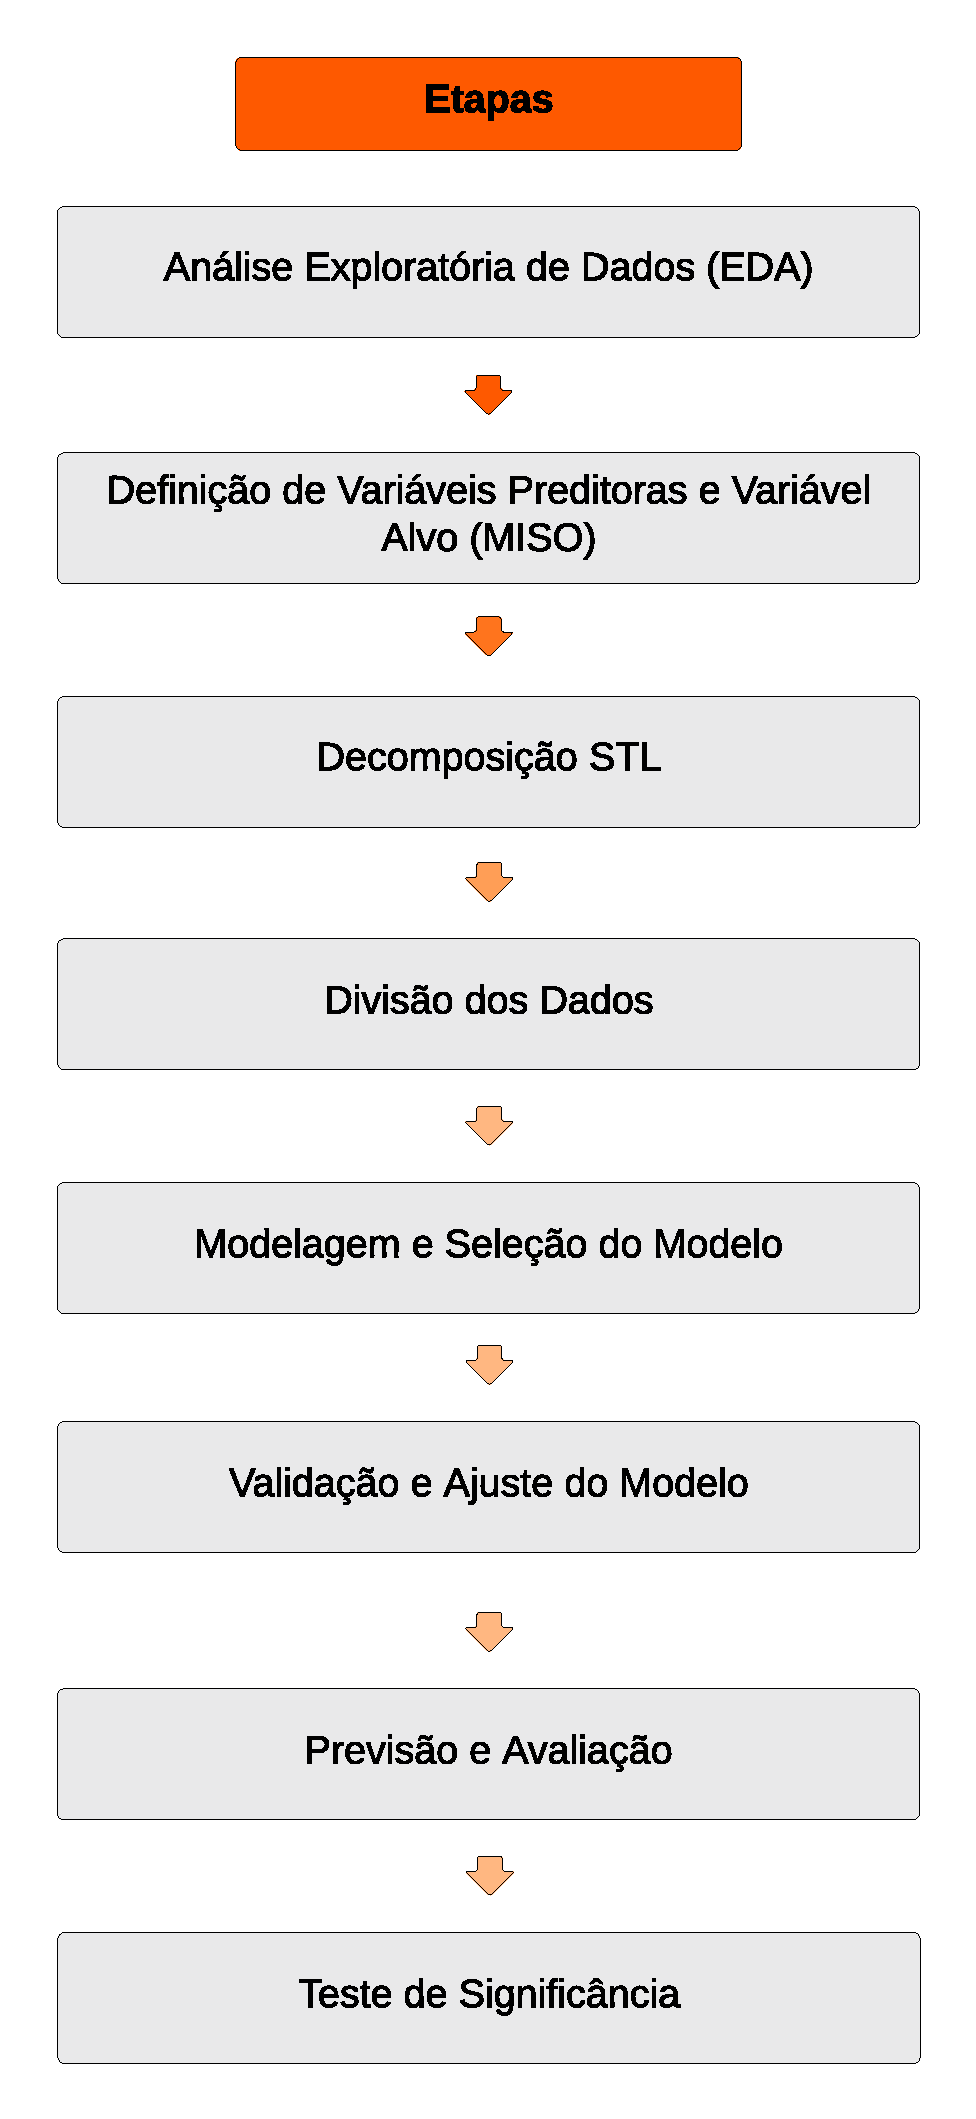
\includegraphics[width=0.7\linewidth]{Introducao/Figuras/Etapas}
\end{figure}

\begin{enumerate}
	
	\item {EDA}: Nesta etapa  tem-se a identificação de valores ausentes, a observação de padrões temporais e a detecção de anomalias. Gráficos de linha são comuns para visualizar a convergência dos dados \cite{Rostam2021108249}.
	
	\item {Definição de Variáveis Preditoras e Variável Alvo (Modelo MISO)}: Na segunda etapa, as variáveis preditoras e a variável alvo para a previsão de Múltiplas Entradas e Uma Saída \textit{Multiple Inputs Single Output} (MISO) são selecionadas. Diferentes modelos, podem incorporar variáveis exógenas na modelagem. Essas variáveis exógenas aprimoram as capacidade de previsão do modelo, especialmente quando o horizonte de previsão se estende além dos dados históricos \cite{PAWLOWSKI202298}. 
	
	\item {Decomposição STL}: O método de decomposição STL separa uma série temporal em três componentes: sazonalidade, tendência e resíduo. Essa decomposição permite. Decompor séries temporais em sazonal captura variações periódicas e repetitivas. Decompor séries temporais em tendência reflete a evolução geral dos dados ao longo do tempo. Para a componente de resíduo engloba as variações não explicadas pelas anteriores \cite{Bandara2021}.
	
	\item {Divisão dos Dados}: É prática comum dividir o conjunto de dados em conjuntos de treinamento, validação e teste para avaliar o desempenho do modelo. Essa divisão permite uma análise da capacidade de generalização dos modelos, evitando problemas de ajuste excessivo ou insuficiente. A proporção de alocação pode variar, mas uma abordagem é alocar 70\% para treinamento e validação, e os 30\% restantes para o conjunto de testes. A porção de treinamento e validação pode ser subdividida em 80\% para treinamento e 20\% para validação \cite{Tao2020}.
	
	\item {Modelagem e Seleção do Modelo}: Nesta etapa, diversos modelos são construídos e avaliados. Alguns modelos comumente usados para previsão de séries temporais incluem ARX, AR, MA, ARIMA, SARIMA, SARIMAX  e modelos de aprendizado de máquina como RNN, LSTM, GRU, DT, LR, XGBoost, LightGBM e Prophet. A escolha do modelo baseia-se em critérios como desempenho na validação, simplicidade do modelo e interpretabilidade dos resultados.
	
	\item {Validação e Ajuste do Modelo}: Durante a construção do modelo, é importante avaliar seu desempenho usando dados de validação. Neste contexto, métricas de avaliação tais como como Erro Médio Absoluto (MAE), Erro Médio Percentual Absoluto Simétrico (SMAPE) e Raiz do Erro Médio Quadrático Relativo (RRMSE) podem ser usadas para comparar e selecionar o melhor modelo. Além disso, técnicas de ajuste como otimização de hiperparâmetros dos modelos usando dados de treinamento e validação combinados podem melhorar o desempenho da previsão das séries temporais.
	
	\item {Previsão e Avaliação}: Com o modelo final com os dados de treinamento e validação, é possível fazer previsões para o conjunto de testes, que representa dados futuros não observados. Essas previsões são comparadas com os valores reais correspondentes para avaliar a qualidade e precisão do modelo.
	
	\item {Teste de Hipótese}: Aplicar os modelos de previsão e fazer comparativo baseado em testes de significância estatística (\textit{Friedman e Nemenjy}).
	
	
	
\end{enumerate}

Cada uma dessas etapas desempenha um papel crucial na análise dos dados e no processo de modelagem das séries temporais, contribuindo para a compreensão dos dados, construção e validação dos modelos de previsão.

\subsection{Estrutura do Documento} \label{subsec:estrutura}

Esse documento de dissertação está organizado em 5 capítulos. O Capítulo~\ref{sec:int}  apresentou contextualização, justificativa, objetivos, contribuições, e a organização do documento.  O Capítulo~\ref{sec:refteo} menciona uma visão geral das principais pesquisas na área de previsão de séries temporais aplicadas a demanda d'água. No Capítulo~\ref{sec:base} são descritos os modelos de previsão que serão utilizados nos dados de séries temporais de abastecimento d'água no Bairro Alto em Curitiba, dados estes fornecidos pela SANEPAR através de coletas horárias durante 3 anos consecutivos. O Capítulo~\ref{sec:result} apresenta os resultados obtidos ao longo da pesquisa com discussões. Os resultados de previsão obtidos são detalhados e a técnica de otimização e métricas estatísticas de desempenho são aplicadas e analisadas. O Capítulo~\ref{sec:conclusoes} apresenta os principais resultados da pesquisa, as limitações e delineia possíveis estudos futuros na área. 
